\documentclass[9pt,letterpaper,onecolumn]{rho-class/rho}
\usepackage[spanish,es-nodecimaldot,es-noindentfirst]{babel}
\usepackage{graphicx}
\usepackage{float}
\setlength{\parindent}{0pt}  % Elimina la sangría
\usepackage[utf8]{inputenc}
\usepackage[T1]{fontenc}
\usepackage{amsmath} % Para la ecuación matemática
\setbool{rho-abstract}{true} % Set false to hide the abstract
\setbool{corres-info}{true} % Set false to hide the corresponding author section
\addbibresource{rho.bib}

%----------------------------------------------------------
% TITLE
%----------------------------------------------------------

%\journalname{Example Template}
\title{TAREA 4: Grape Loot}

%----------------------------------------------------------
% AUTHORS AND AFFILIATIONS
%----------------------------------------------------------
\author[$\dagger$]{Manuel González}
\author[$\dagger$]{Pablo Gómez}
\author[$\dagger$]{Ayrton Morrison}
\author[$\dagger$]{Emmanuel Velásquez}


%----------------------------------------------------------

%\affil[1]{Affiliation of author one}
%\affil[2]{Affiliation of author two}
%\affil[3]{Affiliation of author three}
\affil[$\dagger$]{Universidad de Magallanes}

%----------------------------------------------------------
% DATES
%----------------------------------------------------------

\dates{Este informe fue compilado el \today}

%----------------------------------------------------------
% FOOTER INFORMATION
%----------------------------------------------------------

%\leadauthor{Author last name et al.}
%\footinfo{Creative Commons CC BY 4.0}
\smalltitle{Estructuras de datos}
%\institution{College name}
\theday{\today} %\today

%----------------------------------------------------------
% ARTICLE INFORMATION
%----------------------------------------------------------

%\corres{Provide the corresponding author information and publisher here.}
%\email{example@organization.com.}
%\doi{\url{https://www.doi.org/exampledoi/XXXXXXXXXX}}

%\received{March 20, 2024}
%\revised{April 16, 2024}
%\accepted{April 20, 2024}
%\published{May 21, 2024}

%\license{Rho LaTeX Class \ccLogo\ This document is licensed under Creative Commons CC BY 4.0.}

%----------------------------------------------------------
% ABSTRACT
%----------------------------------------------------------

\begin{abstract}
    En el presente informe técnico se detallará el planteamiento y desarrollo de una red social simplificada, mostrando el uso de algoritmos de similitud, manejo de archivos y uso de estructuras de datos eficientes para esto.
\end{abstract}

%----------------------------------------------------------

\keywords{Estructuras de datos, algoritmos, manejo de archivos}

%----------------------------------------------------------
\begin{document}
    \maketitle
    \thispagestyle{firststyle}
    \tableofcontents
    %\linenumbers
    %----------------------------------------------------------


    \newpage
    \section{Introducción}
La presente tarea tiene como propósito consolidar los conocimientos adquiridos mediante el 	diseño e implementación de un sistema práctico. En esta ocasión, el proyecto se centra en el desarrollo de una red social simulada, un entorno que permitirá implementar y evaluar diversos algoritmos de recomendación y técnicas relacionadas con redes sociales. Este entorno incluye el uso de estructuras de datos avanzadas como grafos y listas enlazadas, integrando también algoritmos como PageRank y la similitud de Jaccard.
El propósito general es simular un sistema que permita realizar recomendaciones basadas en la importancia y similitud de nodos en una red, promoviendo la personalización de las interacciones y resolviendo desafíos técnicos relacionados con la gestión dinámica de datos en estructuras complejas.
    \section{Objetivo principal}
El objetivo principal es diseñar e implementar un sistema funcional que permita gestionar perfiles de usuario, conexiones entre ellos y operaciones asociadas como publicaciones, búsquedas y recomendaciones. Este proyecto busca aplicar conceptos fundamentales de estructuras de datos y algoritmos avanzados para resolver problemas reales relacionados con la gestión y optimización de redes sociales simuladas.
    \newpage
    \section{Planteamiento del desarrollo del proyecto}

    \newpage
    \section{Implementación}

La implementación se desarrolla en etapas:

\begin{itemize}
    \item \textbf{Estructuras de datos:}
    \begin{itemize}
        \item Uso de grafos para modelar las relaciones entre usuarios.
        \item Implementación de listas enlazadas y tablas hash para gestionar datos asociados a cada usuario.
    \end{itemize}

    \item \textbf{Algoritmos:}
    \begin{itemize}
        \item Cálculo de la similitud de Jaccard para sugerencias basadas en intereses comunes.
    \end{itemize}

    \item \textbf{Manejo de datos:}
    \begin{itemize}
        \item Almacenamiento estructurado en directorios para cada usuario.
        \item Archivos separados para guardar seguidores, seguidos y datos generales de los usuarios.
    \end{itemize}

    \item \textbf{Generadores dinámicos:}
    \begin{itemize}
        \item Creación automática y controlada de usuarios.
        \item Generación de conexiones aleatorias y recomendaciones personalizadas.
    \end{itemize}

    \item \textbf{Interfaz de interacción:}
    \begin{itemize}
        \item Desarrollo de una interfaz de línea de comandos para manejar la creación, modificación y búsqueda de usuarios.
        \item Ejecución a través de parámetros para una interacción dinámica.
    \end{itemize}
\end{itemize}

\subsection*{Cálculo de la Similitud de Jaccard}

\begin{itemize}
    \item Para la implementación del índice de Jaccard, se utilizó una tabla hash para las representar las preferencias de cada usuario. Esto maximiza la eficiencia al realizar comparaciones necesarias entre las preferencias de dos usuarios y facilita el cálculo de dicho índice.
\end{itemize}

\subsection*{Creación Automática de Usuarios}

\begin{itemize}
    \item Para la creación automática de usuarios, se creó un modelo matemático que calcula la máxima cantidad de usuarios que podrían crearse según el número de perfiles en la red. Cada cierto intervalo de tiempo, se verifica el número de usuarios en la red y, en base a eso, se calcula la máxima cantidad de perfiles utilizando el siguiente modelo:
\end{itemize}

\[
U_{\text{máx}}(n_0) = \left(\frac{n_0 + 180}{n_0}\right)^{\frac{2}{3}}
\]

donde:
\begin{itemize}
    \item $U_{\text{máx}}$ es la máxima cantidad de usuarios.
    \item $n_0$ es el número de usuarios actual en la red.
\end{itemize}

Después de usar el modelo matemático para limitar la cantidad de usuarios que se puedan crear, se genera un número aleatorio entre \( 0 \) y el valor devuelto por la función. Este número representa la cantidad de usuarios a crear.

\subsection*{Justificación del Modelo Matemático}

\begin{itemize}
    \item El modelo matemático simula el crecimiento controlado de la red social, asegurando que cuando la cantidad de usuarios en la red alcance o supere los \( 100 \), solo se pueda crear un usuario nuevo a la vez. Esto permite que la red crezca de forma continua, pero cada vez más suave.
\end{itemize}

\begin{figure}[h!]
    \centering
    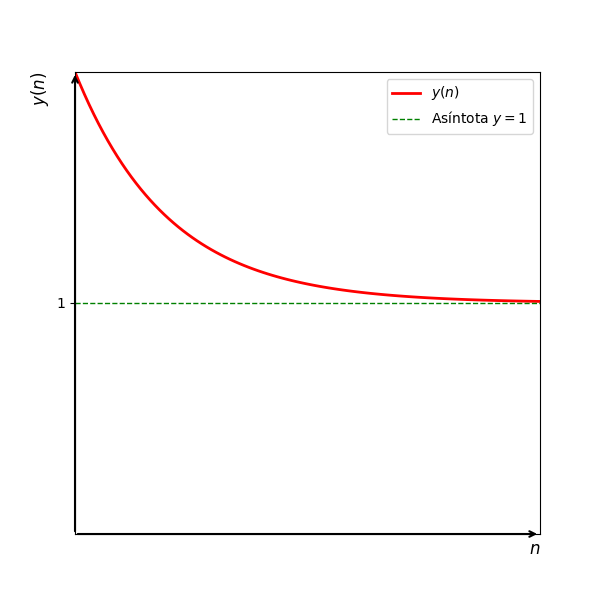
\includegraphics[width=0.5\textwidth]{src/figures/Figure_1.png}
    \caption{Ejemplo.}
    \label{fig:jaccard}
\end{figure}



La creacion del mdoelo se puede explicar en las siguientes expresiones matematicas, en dodne podemos observar el por que esta Modelo toma los comportamientos indicados anteriormente.
\begin{equation}
    \underset{n \to \infty}{\text{Lim}} \quad y(n) = 1 \quad (\text{Asintota horizontal en } y=1)
    %\lim_{n \to \infty} y(n) = 1 \quad (\text{Asintota horizontal en } y=1)
\end{equation}

\begin{equation}
   \left. \frac{dy}{dn} \right|_{n = m} < 0 \quad \forall  m \in \mathbb{R}^+ \quad \text{(Decreciente)}
\end{equation}

\begin{equation}
  U_{\text{máx}}(n) = \left\lfloor y(n) \right\rfloor \quad \text{(Discretizacion del modelo)}
\end{equation}




    \newpage
    \section{Gestión del equipo de trabajo}
El equipo de trabajo está compuesto por los siguientes integrantes: Ayrton Morrison, Emmanuel Velásquez, Manuel González y Pablo Gómez. Los integrantes del equipo se devidieron en dos: Equipo de programación y equipo de documentacion.\\

    \newpage
    \section{Posibles Mejoras a futuro}
En esta sección se describen algunas posibles mejoras que se podrían implementar en el futuro para optimizar y ampliar el proyecto:

\begin{itemize}
    \item \textbf{Optimización del rendimiento:} Revisar y mejorar el código para reducir el tiempo de ejecución y el uso de recursos.
    \item \textbf{Ampliación de funcionalidades:} Añadir nuevas características que puedan ser útiles para los usuarios, basadas en el feedback recibido.
    \item \textbf{Mejora de la documentación:} Asegurarse de que toda la documentación esté actualizada y sea fácil de entender para nuevos desarrolladores.
    \item \textbf{Pruebas automatizadas:} Implementar un conjunto completo de pruebas automatizadas para garantizar la estabilidad y la calidad del código.
    \item \textbf{Interfaz de usuario:} Mejorar la interfaz de usuario para hacerla más intuitiva y fácil de usar.
    \item \textbf{Manejo de memoria:} El programa cuenta con un manejo optimo de memoria, sin embargo aun se presentan ciertas fugas al liberar la memoria utilizada, si bien no es demasiado, es importante tenerlo en cuenta para una futura implementación.
\end{itemize}
    \newpage
    \section{Ejemplo de uso}

    \newpage
    \section{Conclusiones}


    \newpage
    %\nocite{*}
    %\printbibliography
\end{document}